% Options for packages loaded elsewhere
\PassOptionsToPackage{unicode}{hyperref}
\PassOptionsToPackage{hyphens}{url}
%
\documentclass[
  12pt,
  a4paper]{extarticle}
\usepackage{amsmath,amssymb}
\usepackage{lmodern}
\usepackage{iftex}
\ifPDFTeX
  \usepackage[T1]{fontenc}
  \usepackage[utf8]{inputenc}
  \usepackage{textcomp} % provide euro and other symbols
\else % if luatex or xetex
  \usepackage{unicode-math}
  \defaultfontfeatures{Scale=MatchLowercase}
  \defaultfontfeatures[\rmfamily]{Ligatures=TeX,Scale=1}
\fi
% Use upquote if available, for straight quotes in verbatim environments
\IfFileExists{upquote.sty}{\usepackage{upquote}}{}
\IfFileExists{microtype.sty}{% use microtype if available
  \usepackage[]{microtype}
  \UseMicrotypeSet[protrusion]{basicmath} % disable protrusion for tt fonts
}{}
\makeatletter
\@ifundefined{KOMAClassName}{% if non-KOMA class
  \IfFileExists{parskip.sty}{%
    \usepackage{parskip}
  }{% else
    \setlength{\parindent}{0pt}
    \setlength{\parskip}{6pt plus 2pt minus 1pt}}
}{% if KOMA class
  \KOMAoptions{parskip=half}}
\makeatother
\usepackage{xcolor}
\IfFileExists{xurl.sty}{\usepackage{xurl}}{} % add URL line breaks if available
\IfFileExists{bookmark.sty}{\usepackage{bookmark}}{\usepackage{hyperref}}
\hypersetup{
  pdftitle={Getting started with accessible maths},
  pdfauthor={Emma Cliffe, Skills Centre: MASH, University of Bath. JISC Accessibility drop-in clinic, June 2022},
  pdflang={en},
  hidelinks,
  pdfcreator={LaTeX via pandoc}}
\urlstyle{same} % disable monospaced font for URLs
\usepackage[margin=2.5cm]{geometry}
\usepackage{longtable,booktabs,array}
\usepackage{calc} % for calculating minipage widths
% Correct order of tables after \paragraph or \subparagraph
\usepackage{etoolbox}
\makeatletter
\patchcmd\longtable{\par}{\if@noskipsec\mbox{}\fi\par}{}{}
\makeatother
% Allow footnotes in longtable head/foot
\IfFileExists{footnotehyper.sty}{\usepackage{footnotehyper}}{\usepackage{footnote}}
\makesavenoteenv{longtable}
\usepackage{graphicx}
\makeatletter
\def\maxwidth{\ifdim\Gin@nat@width>\linewidth\linewidth\else\Gin@nat@width\fi}
\def\maxheight{\ifdim\Gin@nat@height>\textheight\textheight\else\Gin@nat@height\fi}
\makeatother
% Scale images if necessary, so that they will not overflow the page
% margins by default, and it is still possible to overwrite the defaults
% using explicit options in \includegraphics[width, height, ...]{}
\setkeys{Gin}{width=\maxwidth,height=\maxheight,keepaspectratio}
% Set default figure placement to htbp
\makeatletter
\def\fps@figure{htbp}
\makeatother
\setlength{\emergencystretch}{3em} % prevent overfull lines
\providecommand{\tightlist}{%
  \setlength{\itemsep}{0pt}\setlength{\parskip}{0pt}}
\setcounter{secnumdepth}{5}
\ifLuaTeX
\usepackage[bidi=basic]{babel}
\else
\usepackage[bidi=default]{babel}
\fi
\babelprovide[main,import]{english}
% get rid of language-specific shorthands (see #6817):
\let\LanguageShortHands\languageshorthands
\def\languageshorthands#1{}
\ifLuaTeX
  \usepackage{selnolig}  % disable illegal ligatures
\fi

\title{Getting started with accessible maths}
\author{Emma Cliffe, Skills Centre: MASH, University of Bath. JISC Accessibility drop-in clinic, June 2022}
\date{}



%\usepackage[english,shorthands=off]{babel}
\usepackage{etoolbox}
\usepackage{spverbatim}
\makeatletter
\@ifpackageloaded{float}{}{\usepackage{float}}
\@ifpackageloaded{adjustbox}{}{\usepackage[Export]{adjustbox}}
\makeatother
\floatplacement{figure}{H}
\newcommand{\scalefactor}{1.2}
\adjustboxset*{min width=\scalefactor\width,max width=\linewidth}
\renewcommand{\familydefault}{phv}
\fontfamily{phv}\selectfont
\renewcommand{\em}{\bf}\renewcommand{\textit}{\textbf}\renewcommand{\emph}{\textbf}\renewcommand{\it}{\bf}\renewcommand{\itshape}{\bf}
\setlength{\parindent}{0.0pt}
\setlength{\parskip}{1.0\baselineskip}
\renewcommand{\baselinestretch}{1.5}\selectfont
\setlength{\mathsurround}{0.2em}
\setlength{\arraycolsep}{0.5cm}\renewcommand{\arraystretch}{1.5}
\addtolength{\jot}{\baselineskip}
\renewcommand{\;}{\,}
\sloppy
\allowdisplaybreaks
\usepackage{amsthm}
\newtheoremstyle{plain}{20pt}{3pt}{}{}{\bfseries}{.\newline\nobreak}{1.0em\nobreak}{}
\newtheoremstyle{definition}{20pt}{3pt}{}{}{\bfseries}{.\newline\nobreak}{1.0em\nobreak}{}
\newtheoremstyle{remark}{20pt}{3pt}{}{}{\bfseries}{.\newline\nobreak}{1.0em\nobreak}{}
\csundef{Proof}
\csundef{endProof}
\newenvironment{Proof}
  {\noindent{\bf Proof.}\hspace*{1em}}% Begin
  {\qed\par}% End
%% When redefining an environment it is vital that it has 
%% the same number of arguments as the original
\renewenvironment{proof}[1][\proofname]
  {\trivlist\item\relax\noindent{\bf {#1}.}\hspace*{1em}}% Begin
  {\qed\endtrivlist}% End

\begin{document}
\maketitle

{
\setcounter{tocdepth}{2}
\tableofcontents
}
\newpage
\pagenumbering{arabic}

\hypertarget{the-plan}{%
\section*{The plan}\label{the-plan}}
\addcontentsline{toc}{section}{The plan}

\begin{itemize}
\tightlist
\item
  What is the problem?
\item
  What to we convert \textbf{\emph{to}}?
\item
  How do we get started?
\end{itemize}

\hypertarget{what-is-the-problem}{%
\section{What is the problem?}\label{what-is-the-problem}}

\hypertarget{could-we-solve-it-by}{%
\subsection{Could we solve it by\ldots?}\label{could-we-solve-it-by}}

You might ask, can we not solve this by ensuring that the PDF is accessible? Unfortunately, the answer is no. The act of creating the PDF destroys information about the structure of the mathematical expression.

\includegraphics[width=0.6\textwidth,height=\textheight]{./reflowing.png}

\hypertarget{computers-and-maths}{%
\subsection{Computers and maths}\label{computers-and-maths}}

\begin{itemize}
\tightlist
\item
  Computers rely on structural integrity to process maths:

  \begin{itemize}
  \tightlist
  \item
    PDF, print, handwriting and E-books using images of maths cannot be processed. They are inaccessible and inflexible on, for instance, small screen devices. They are lossy formats for maths!
  \item
    Word, HTML based formats and EPub3 have structural integrity for maths and are accessible to many assistive technologies (AT)
  \item
    But not all AT can access maths all formats! PowerPoint 365 is theoretically accessible but most AT won't work with it
  \end{itemize}
\item
  Using a computer with or without assistive technology to write mathematics is a specialist skill!
\item
  Using AT effectively for maths requires authors to produce accessible materials which is challenging due to how mathematicians and scientists typically produce text and documents.
\end{itemize}

\hypertarget{from-retrofitting-to-inclusive-design}{%
\subsection{From retrofitting to inclusive design?}\label{from-retrofitting-to-inclusive-design}}

I have spent the last 18 years trying to retrofit accessible interfaces to the entirely natural community evolved handwritten, typeset and old software based maths learning environments.

It is important to understand that this is a side effect of a more general difficulty - mathematicians continue to hand write and then, maybe, typeset for a reason!

But, we relied on expertise at the intersection of higher level maths, programming and access. Retrofitting is an expensive, inefficient compromise reliant on rare skill sets, research output organically grown tools and, to be honest, serendipity!

\hypertarget{could-we-convert-the-latex}{%
\subsection{Could we convert the LaTeX?}\label{could-we-convert-the-latex}}

\begin{itemize}
\tightlist
\item
  It depends on the LaTeX\ldots{}
\item
  The past: use \href{https://hub.docker.com/r/bathmash/mathaltnotes}{tools which may or may not work and that cannot tell you, in general why something doesn't work created and driven by specialists}
\item
  The future? \href{https://ctan.org/pkg/lwarp?lang=en}{lwarp} but beware of some hard work (documentation currently 1237 pages) - what happens depends on what you are doing in LaTeX and how and you have to work that out and test for accessibility for yourself.
\item
  It is \textbf{not possible} to convert LaTeX to html in the general case.
\end{itemize}

\hypertarget{could-we-convert-the-mathematicians}{%
\subsection{Could we convert the mathematicians?!}\label{could-we-convert-the-mathematicians}}

Any new document preparation system needs to \textbf{\emph{enable}} the writer by providing the key features of mathematical/scientific document preparation. And these features make things complex.

\begin{itemize}
\tightlist
\item
  Software is catching up and in flux.
\item
  Nothing is easy to learn.
\end{itemize}

Increasingly mathematicians are exploring and converting, but they need appropriate institutional infrastructure, support, workload time allocation and training. Without this the task remains unreasonable.

\hypertarget{what-do-we-convert-to}{%
\section{\texorpdfstring{What do we convert \textbf{\emph{to}}?}{What do we convert to?}}\label{what-do-we-convert-to}}

From a technical point of view there are only three formats of mathematical text which are accessible:

\begin{itemize}
\tightlist
\item
  Word
\item
  HTML using MathJax to render the mathematics
\item
  EPub3
\end{itemize}

Supply at least one or, ideally, all (some AT can only access one format, EPub3 has least software support).

\textbf{But} you also need to supply PDF!

\begin{itemize}
\tightlist
\item
  Not all accessibility is about technical access
\item
  Clear print PDF is selected most often by disabled students in the Department of Mathematical Sciences.
\end{itemize}

\hypertarget{how-do-we-get-started}{%
\section{How do we get started?}\label{how-do-we-get-started}}

\hypertarget{word-365-accessibility-checker-equation-editor}{%
\subsection{Word 365: Accessibility checker + Equation editor}\label{word-365-accessibility-checker-equation-editor}}

\begin{itemize}
\tightlist
\item
  Use the inbuilt Word Accessibility Checker and information on \href{https://support.office.com/en-gb/article/make-your-word-documents-accessible-to-people-with-disabilities-d9bf3683-87ac-47ea-b91a-78dcacb3c66d}{Making your Word documents accessible}
\item
  Write \emph{all} mathematical text written using the Word 365 equation editor. E.g. if you are writing about the variable \(x\) or \(\theta\) it should be written as an equation. If you are writing \(x^2\) it should be written as an equation.

  \begin{itemize}
  \tightlist
  \item
    Never use insert symbol.
  \item
    Never write superscripts, subscripts, fractions etc. using font or style changes and standard keyboard input alone
  \item
    Never use an image of an equation.
  \end{itemize}
\item
  Use Review -\textgreater{} Read Aloud (Alt + Ctrl + Space) to check the maths
\end{itemize}

More information and tools within \href{https://stem-enable.github.io/WordWorkshop/}{accessible mathematical Word document workshop resources} and \href{https://bathmash.github.io/gettingstarted/Word/index.html}{effective (keyboard-only) input of maths in Word}.

\hypertarget{sounds-solved-to-me}{%
\subsection{Sounds solved to me?}\label{sounds-solved-to-me}}

Some students will require MathType format

\begin{itemize}
\tightlist
\item
  Because their AT vendor has not implemented the interface to Word but the AT does work with MathType. Test everything and contact the vendors!
\item
  Materials should be prepared as above and then a \textbf{\emph{copy}} converted to MathType as automatic conversion of all expressions cannot be reversed.
\end{itemize}

Also\ldots{} this generally won't work for the mathematicians and some scientists.

\begin{itemize}
\tightlist
\item
  Word is not a scientific document preparation system.
\item
  For those who use LaTeX we need a different plan.
\end{itemize}

\hypertarget{web-wcag-2.1-aa-mathjax}{%
\subsection{Web: WCAG 2.1 AA + MathJax!}\label{web-wcag-2.1-aa-mathjax}}

\begin{itemize}
\item
  Check it meets the legal requirement of WCAG 2.1 Level AA with e.g.~\href{https://accessibilityinsights.io/docs/en/web/overview}{Accessibility Insights for Web plugin for Chrome}
\item
  Check it is MathJax\ldots{} Right click!
  \[x = \frac{-b\pm\sqrt{b^2 - 4ac}}{2a}\]

  \begin{itemize}
  \tightlist
  \item
    Provides/enables: navigation, chunking, zoom, copy/paste, colour, size and layout changes\ldots{}
  \item
    Structural integrity enables assistive technology including text-to-speech, screenreaders, electronic Braille
  \item
    Fallback for ARIA-aware AT without native support
  \item
    AT providers without native support and not ARIA aware are a problem but not your problem.
  \end{itemize}
\end{itemize}

\hypertarget{moodle-support-throughout}{%
\subsection{Moodle support throughout!}\label{moodle-support-throughout}}

Moodle enables you to create pages which meet these requirements using LaTeX for the equations.

\textbf{But} Moodle does not provide the necessary features of a mathematical/scientific document preparation system.

\begin{itemize}
\tightlist
\item
  Web + MathJax is the most accessible end format for a mathematical or scientific document but we need a way to prepare the document
\end{itemize}

\hypertarget{supporting-mathematicians}{%
\subsection{Supporting mathematicians}\label{supporting-mathematicians}}

We are not perscriptive but recommend RMarkdown. We'll support anything which helps them do the job though.

\begin{itemize}
\tightlist
\item
  RMarkdown incorporates LaTeX for equations and a simple markup language for the rest of the document.
\item
  Authors are confined to a transformable subset with a quick compile loop and a supportive GUI.
\item
  The output has known accessibility features.
\item
  The typesetting is still extensible, just more reasonably so.
\end{itemize}

More information on getting started \href{https://stem-enable.github.io/RMarkdownWorkshop/}{RMarkdown workshop resources}

\begin{itemize}
\tightlist
\item
  \href{https://bookdown.org/}{Bookdown} needed for theorems and intradocument referencing
\item
  \href{https://bathmash.github.io/clavertondown/}{Clavertondown} for additional functionality important in pure mathematics and for lecturers generally
\end{itemize}

\hypertarget{thanks-for-listening-and-watching}{%
\section{Thanks for listening and watching}\label{thanks-for-listening-and-watching}}

\begin{itemize}
\tightlist
\item
  This document is available at \href{https://stem-enable.github.io/Getting-started-with-accessible-maths/index.html}{Getting started with accessible maths}
\item
  My email address is \href{mailto:E.H.Cliffe@bath.ac.uk}{\nolinkurl{E.H.Cliffe@bath.ac.uk}}
\item
  A collection of links to most things I have done related to maths accessibility can be found at \href{https://www.bath.ac.uk/projects/mathematics-accessibility/}{Mathematics accessibility on the Skills Centre: MASH site}
\end{itemize}

\hypertarget{mathematical-diagrams-software-and-interactivedynamic-elements-including-e-assessment}{%
\subsection{Mathematical diagrams, software and interactive/dynamic elements including e-assessment}\label{mathematical-diagrams-software-and-interactivedynamic-elements-including-e-assessment}}

This won't be covered in the talk but is here in case it is useful!

\begin{itemize}
\tightlist
\item
  Check that the software/system meets WCAG 2.1 level AA - ask the vendor, procure on this basis

  \begin{itemize}
  \tightlist
  \item
    Be aware that many mathematical and statistical analysis systems are still not accessible
  \end{itemize}
\item
  Check that mathematics is rendered via MathJax
\item
  Start to use emerging tools which have known accessibility status for creation of dynamic elements:

  \begin{itemize}
  \tightlist
  \item
    Desmos, BrailleR, Geogebra (with care)
  \item
    Numbas, Stack
  \end{itemize}
\item
  If you made a diagram using data or code or some textbased input mechanism then provide that text or link to it somehow.
\item
  Learn to describe diagrams which can't currently be replaced:

  \begin{itemize}
  \tightlist
  \item
    DIAGRAM Center (\url{http://diagramcenter.org/}):

    \begin{itemize}
    \tightlist
    \item
      Poet Image Description Training Tool
    \item
      Image description guidelines
    \item
      Sample book
    \item
      Webinar: \url{http://diagramcenter.org/diagramwebinars.html\#compleximages}
    \end{itemize}
  \item
    UKAAF has guidance on accessible images: \url{https://www.ukaaf.org/standards/\#accessible-images}
  \item
    NCAM (Old site) has guidelines and examples: \url{http://ncamftp.wgbh.org/ncam-old-site/experience_learn/educational_media/stemdx.html}
  \end{itemize}
\end{itemize}

\hypertarget{example-desmos}{%
\subsubsection{Example: Desmos}\label{example-desmos}}

\href{https://www.desmos.com/accessibility}{Desmos produces interactive graphs, is screenreader accessible and can also produces tactile diagrams}. If you can redraw the graph in Desmos then do that! Try the below with a screenreader.

\includegraphics[width=0.3\textwidth,height=\textheight]{./desmos-sine-graph.png}

\hypertarget{example-brailler}{%
\subsubsection{Example: BrailleR}\label{example-brailler}}

If you are making some sorts of statistical graphs and you know how to use R (fairly well) then there is a \href{https://github.com/ajrgodfrey/BrailleR}{BrailleR} package which can create descriptions of some sorts of graphs automatically.

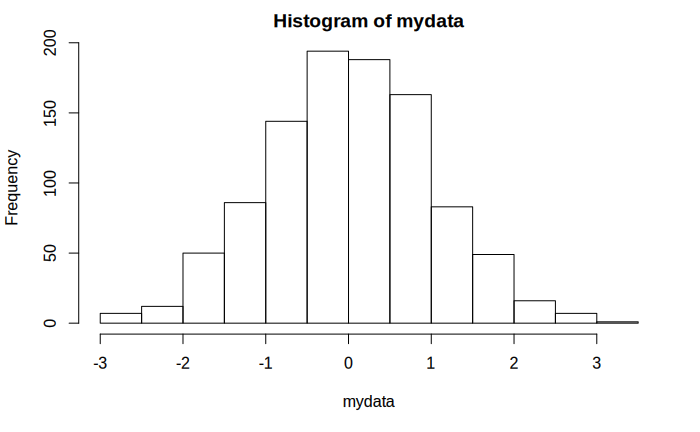
\includegraphics[width=\Width,height=\Height]{./Figs/myhist2.svg.pdf}

\end{document}
